\documentclass[11pt, a4paper]{article}

\usepackage{amsmath}
\usepackage{amsfonts} %Matheschriften
\usepackage{amssymb} %Mathesymbole
%\usepackage{mathptmx} % Einstellung für Schriften und Sonderzeichen in mathematischen Umgebungen
                        % ändert SChriftfont
\usepackage{wasysym} % Stellt diverse Sonderzeichen bereit
\usepackage{siunitx}
\usepackage{float}
\usepackage{microtype}
\usepackage{graphicx}
\usepackage{hyperref}
\usepackage{xcolor}
\usepackage[section]{placeins}
% allows for temporary adjustment of side margins
\usepackage{changepage}
\usepackage{rotating}


\usepackage[ngerman]{babel}
\addto\captionsngerman{%
 \renewcommand{\abstractname}{Einleitung}}

\title{Versuch 5: Franz Herz Versuch}
\author{Team 4-11: Jascha Fricker, Benedict Brouwer}

\DeclareSIUnit\electron{e}

\begin{document}
    \maketitle

    \tableofcontents

    \newpage

    \section{Einleitung}
    Der Franck-Hertz-Versuch ist ein wichtiger Versuch in der Atomphysik, der von James Franck und Gustav Hertz durchgeführt wurde1. Der Versuch belegt die Existenz von diskreten Energieniveaus in Atomen und stützt das bohrsche Atommodell. Die Experimente wurden 1914 veröffentlicht und 1922 mit dem Nobelpreis für Physik ausgezeichnet.

    \section{Theorie}

    Die Elektronen beschleunigten können gebundene Elektronen im Gas in höheren Bahnen haben. Die Bahnen sind durch den Bahndrehimpuls
    \begin{equation}
        L = \hbar n
    \end{equation}
    gequantelt. Wenn die Elektronen wieder in ihre ursprünglichen Bahnen zurückfallen, dann werden Photonen mit der Frequenz
    \begin{equation}
        h \cdot f = E_1 - E_2 = h \cdot \frac{c}{\lambda} \label{eq:energie}
    \end{equation}
    freigesetzt. Die Energieniveaus der zwei Gase Hg und Neon sind in den Abbildungen \ref{fig:Hgenergie} und \ref{fig:Neonenergie} dargestellt.

    \begin{figure}[h]
        \centering
        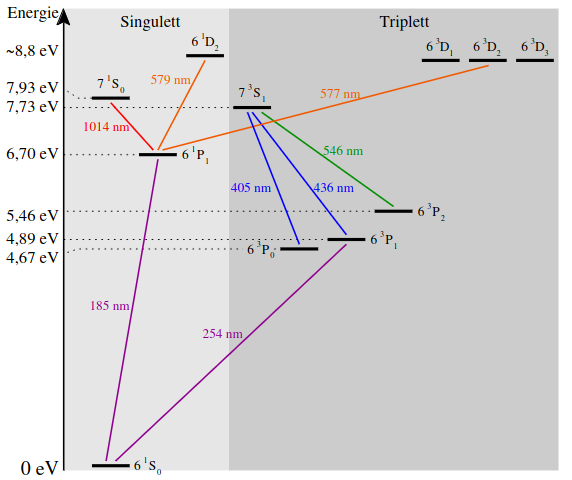
\includegraphics[width=0.5\textwidth]{Screenshot_20230320_160508.png}
        \caption{Energieniveaus von Hg \cite{FHV}}
        \label{fig:Hgenergie}
    \end{figure}

    \begin{figure}[h]
        \centering
        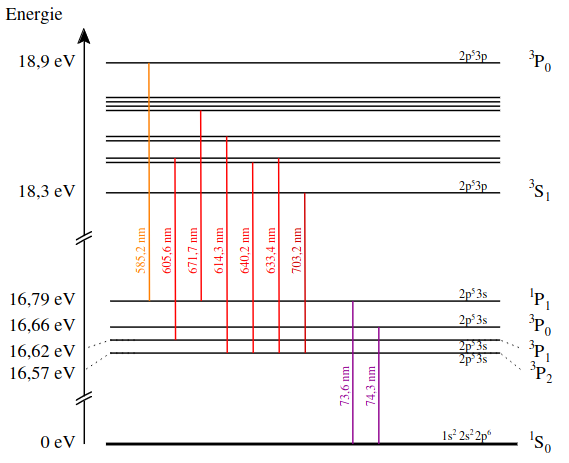
\includegraphics[width=0.5\textwidth]{Screenshot_20230320_160547.png}
        \caption{Energieniveaus von Neon \cite{FHV}}
        \label{fig:Neonenergie}
    \end{figure}

    \section{Versuchsaufbau und Durchführung}

    Der Versuchsaufbau ist in Abbildung \ref{fig:Versuchsaufbau} gezeigt und besteht aus einer Röhre die mit dem jeweilligen Stoff gefüllt ist. Bei Queckssilber muss diese durch einen Ofen erhitzt werden, damit das Quecksilber gasförmig wird. Zwischen der Anode und Kathode wird eine Spannung angelegt, um die Elektronen zu breschleunigen. Mit dem Betriebsgerät wird auch eine kleine negative Spannung an die Auffangelektrode angelegt und dann gemessen, wie viele Elektronen auf die Auffangelektrode treffen, indem der Strom gemessen wird. Durch diesen Auffängerstrom abhängig vom der Beschleunigungsspannung zu beobachten, können dann Rückschlüsse auf die Vorgänge in der Röhre gezogen werden.

    \begin{figure}[h]
        \centering
        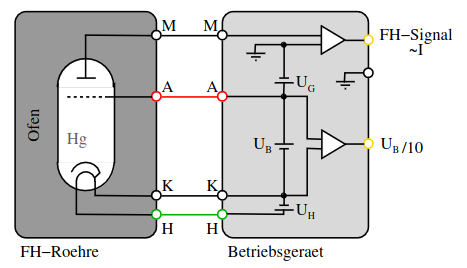
\includegraphics[width=0.5\textwidth]{Screenshot_20230320_160645.png}
        \caption{Versuchsaufbau Hg \cite{FHV}}
        \label{fig:Versuchsaufbau}
    \end{figure}

    \section{Ergebnisse}

    \subsection{Queckssilber}

    Der Gewichtete Mittelwert der Spannungsdifferenzen der Maxima bzw Minima beträgt $E = 4,93(28) \si{\electron\volt}$. Daraus lässt sich eine Wellenlänge von 
    \begin{equation}
        \lambda = \frac{h \cdot c}{E} = 252(14) \si{\nano\meter}
    \end{equation}
    berechnen. Dies passt genau mit dem Übergang von $6^3\text{P}_1$ zu $6^1\text{S}_0$ mit $254 \si{\nano\meter}$ \ref{fig:Hgenergie} überein.
    Die Unsicherheit der Spannung wurde mithilfe der Tabelle 4 des ABW-Skripts \cite{ABW} berechnet. Als Bremsspannung wurde $U_B = 1,72 \si{\volt}$ und als Heizspannung $U_H = 9,51 \si{\volt}$ verwendet.

    \subsection{Neon}

    Der Gewichtete Mittelwert der Spannungsdifferenzen der Maxima bzw Minima beträgt $E = 20,2(11) \si{\electron\volt}$. Daraus lässt sich eine theoretische Wellenlänge von $61,5(35) \si{\nano\meter}$ berechnen. Diese wird aber nicht in einem mal ausgesandt, sondern in mehreren Linien. Die Energie weicht etwas vom Literaturwert von 18,3 eV und 18,9 eV ab \cite{FHV}. Das liegt wahrscheinlich an der sehr begrenzten Anzahl an Messungen.
    Als Bremsspannung wurde $U_B = 8,67 \si{\volt}$ und als Heizspannung $U_H = 4,35 \si{\volt}$ verwendet.
    Mit dem Spektrometer konnten Linien bei $590 \si{\nano\meter}$, $620 \si{\nano\meter}$ und $650 \si{\nano\meter}$ gemessen werden. Infrage kommen die Spektrallinien bei $585,2 \si{\nano\meter}$, $614,3 \si{\nano\meter}$ und $640,2 \si{\nano\meter}$ aus der Abbildung \ref{fig:Neonenergie}.
    \bibliographystyle{plain}
    \bibliography{literature}

\end{document}